\documentclass[border=5pt]{standalone}
\usepackage{tikz}
\usetikzlibrary{calc, positioning}
\usepackage{amsmath}
\begin{document}
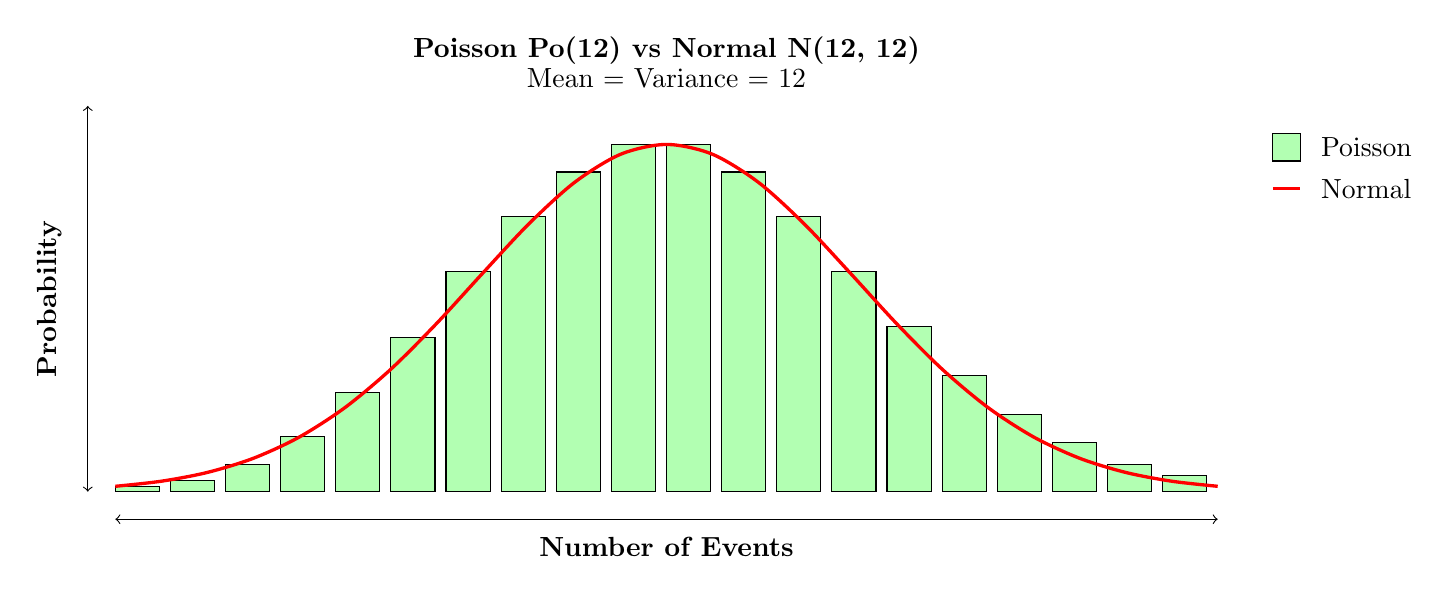
\begin{tikzpicture}[scale=0.7]
% Poisson histogram bars (manually calculated approximate values)
\draw[fill=green!30, draw=black] (2, 0) rectangle (2.8, 0.1);
\draw[fill=green!30, draw=black] (3, 0) rectangle (3.8, 0.2);
\draw[fill=green!30, draw=black] (4, 0) rectangle (4.8, 0.5);
\draw[fill=green!30, draw=black] (5, 0) rectangle (5.8, 1.0);
\draw[fill=green!30, draw=black] (6, 0) rectangle (6.8, 1.8);
\draw[fill=green!30, draw=black] (7, 0) rectangle (7.8, 2.8);
\draw[fill=green!30, draw=black] (8, 0) rectangle (8.8, 4.0);
\draw[fill=green!30, draw=black] (9, 0) rectangle (9.8, 5.0);
\draw[fill=green!30, draw=black] (10, 0) rectangle (10.8, 5.8);
\draw[fill=green!30, draw=black] (11, 0) rectangle (11.8, 6.3);
\draw[fill=green!30, draw=black] (12, 0) rectangle (12.8, 6.3);
\draw[fill=green!30, draw=black] (13, 0) rectangle (13.8, 5.8);
\draw[fill=green!30, draw=black] (14, 0) rectangle (14.8, 5.0);
\draw[fill=green!30, draw=black] (15, 0) rectangle (15.8, 4.0);
\draw[fill=green!30, draw=black] (16, 0) rectangle (16.8, 3.0);
\draw[fill=green!30, draw=black] (17, 0) rectangle (17.8, 2.1);
\draw[fill=green!30, draw=black] (18, 0) rectangle (18.8, 1.4);
\draw[fill=green!30, draw=black] (19, 0) rectangle (19.8, 0.9);
\draw[fill=green!30, draw=black] (20, 0) rectangle (20.8, 0.5);
\draw[fill=green!30, draw=black] (21, 0) rectangle (21.8, 0.3);

% Normal curve overlay N(12, 12)
\draw[red, very thick] plot[smooth, domain=2:22] (\x, {6.3*exp(-(\x-12)^2/(2*12))});

% Labels and annotations
\draw[<->] (2, -0.5) -- (22, -0.5);
\node at (12, -1) {\textbf{Number of Events}};
\draw[<->] (1.5, 0) -- (1.5, 7);
\node[rotate=90] at (0.8, 3.5) {\textbf{Probability}};
\node at (12, 8) {\textbf{Poisson Po(12) vs Normal N(12, 12)}};
\node at (12, 7.5) {Mean = Variance = 12};

% Legend
\draw[fill=green!30, draw=black] (23, 6) rectangle (23.5, 6.5);
\node[right] at (23.7, 6.25) {Poisson};
\draw[red, very thick] (23, 5.5) -- (23.5, 5.5);
\node[right] at (23.7, 5.5) {Normal};
\end{tikzpicture}
\end{document}
